\begin{figure}
\centering

\begin{subfigure}[b]{0.34\textwidth}
\centering


\scalebox{0.58}{
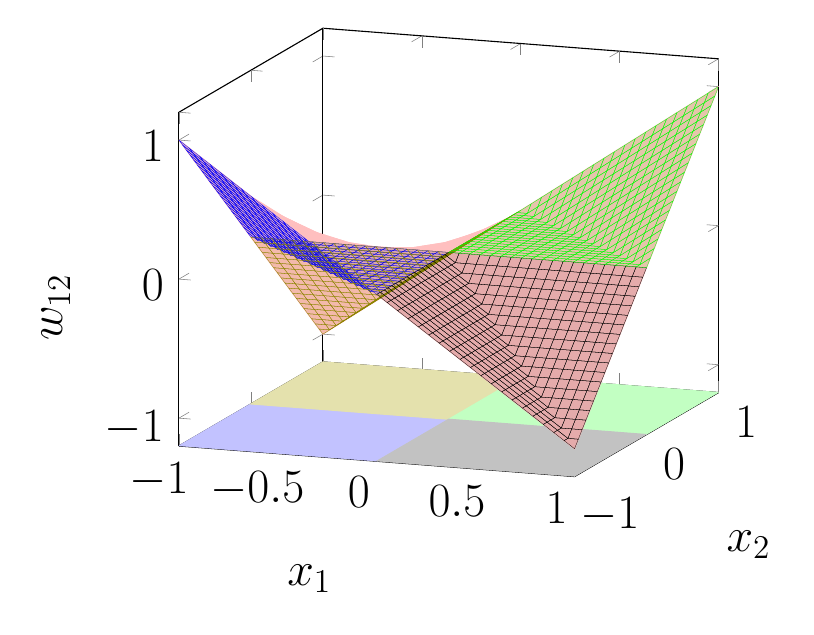
\begin{tikzpicture}
 
\LARGE
\begin{axis}[view = {20}{15}, 
xlabel=$x_1$,
ylabel=$x_2$,
zlabel={$w_{12}$},
    area plot/.style={
        fill opacity=0.1,
        ultra thin,
        fill=blue!70,
        mark=none,
        smooth
    }]

\filldraw[blue!24] plot coordinates{(-1,-1,-1.2) (-1,0,-1.2) (0,0,-1.2) (0,-1,-1.2)}--cycle;

\filldraw[olive!24] plot coordinates{(-1,0,-1.2) (-1,1,-1.2) (0,1,-1.2) (0,0,-1.2)}--cycle;

\filldraw[green!24] plot coordinates{(0,0,-1.2) (0,1,-1.2) (1,1,-1.2) (1,0,-1.2)}--cycle;

\filldraw[black!24] plot coordinates{(0,-1,-1.2) (0,0,-1.2) (1,0,-1.2) (1,-1,-1.2)}--cycle;
 
\addplot3 [
    domain=-1:1,
    domain y = -1:1,
    samples = 10,
    samples y = 10,
    surf,
    fill=pink,
    faceted color = pink] {x*y};
    

\addplot3 [area plot,
    domain=-1:0,
    domain y = -1:0,
    samples = 20,
    samples y = 20,
    surf,
    fill=blue,
    faceted color = blue] {max(0, -x-y-1)};
    

\addplot3 [area plot,
    domain=-1:0,
    domain y = 0:1,
    samples = 20,
    samples y = 20,
    surf,
    fill=olive,
    faceted color = olive] {max(x, -y)};
    

\addplot3 [area plot,
    domain=0:1,
    domain y = -1:0,
    samples = 20,
    samples y = 20,
    surf,
    fill=black,
    faceted color = black] {max(-x, y)};
    

\addplot3 [area plot,
    domain=0:1,
    domain y = 0:1,
    samples = 20,
    samples y = 20,
    surf,
    fill=green,
    faceted color = green] {max(0, x+y-1)};
    
    
 
\end{axis}
 
\end{tikzpicture}
}


% \caption{Lower part of the piecewise McCormick relaxation for a bilinear term}
\end{subfigure}
\hfill
\begin{subfigure}[b]{0.34\textwidth}
\centering


\scalebox{0.58}{
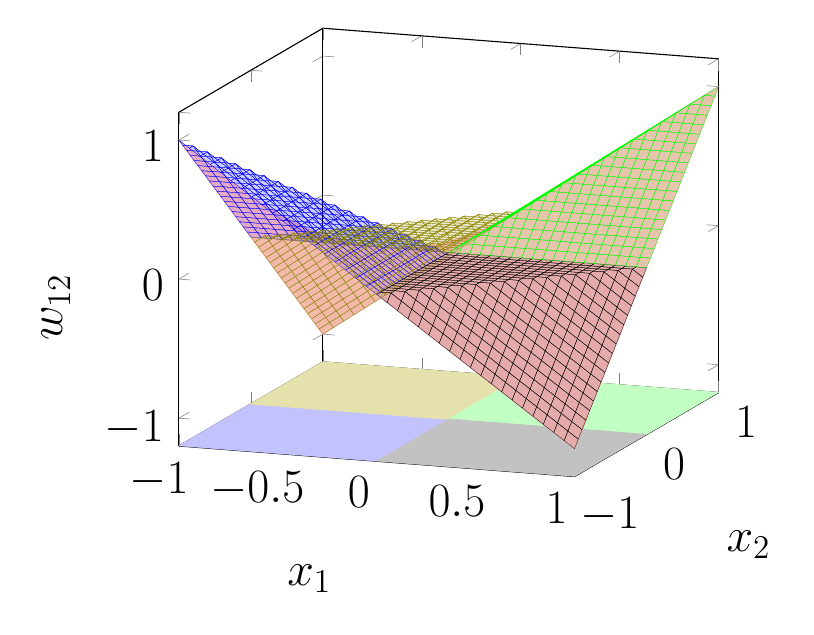
\begin{tikzpicture}
 
\LARGE

\begin{axis}[view = {20}{15}, 
xlabel=$x_1$,
ylabel=$x_2$,
zlabel={$w_{12}$},
    area plot/.style={
        fill opacity=0.1,
        ultra thin,
        fill=blue!70,
        mark=none,
        smooth
    }]

\filldraw[blue!24] plot coordinates{(-1,-1,-1.2) (-1,0,-1.2) (0,0,-1.2) (0,-1,-1.2)}--cycle;

\filldraw[olive!24] plot coordinates{(-1,0,-1.2) (-1,1,-1.2) (0,1,-1.2) (0,0,-1.2)}--cycle;

\filldraw[green!24] plot coordinates{(0,0,-1.2) (0,1,-1.2) (1,1,-1.2) (1,0,-1.2)}--cycle;

\filldraw[black!24] plot coordinates{(0,-1,-1.2) (0,0,-1.2) (1,0,-1.2) (1,-1,-1.2)}--cycle;
 
\addplot3 [
    domain=-1:1,
    domain y = -1:1,
    samples = 10,
    samples y = 10,
    surf,
    fill=pink,
    faceted color = pink] {x*y};
    

\addplot3 [area plot,
    domain=-1:0,
    domain y = -1:0,
    samples = 20,
    samples y = 20,
    surf,
    fill=blue,
    faceted color = blue] {min(-x, -y)};
    

\addplot3 [area plot,
    domain=-1:0,
    domain y = 0:1,
    samples = 20,
    samples y = 20,
    surf,
    fill=olive,
    faceted color = olive] {min(0, x-y+1)};
    

\addplot3 [area plot,
    domain=0:1,
    domain y = -1:0,
    samples = 20,
    samples y = 20,
    surf,
    fill=black,
    faceted color = black] {min(0, y-x+1)};
    

\addplot3 [area plot,
    domain=0:1,
    domain y = 0:1,
    samples = 20,
    samples y = 20,
    surf,
    fill=green,
    faceted color = green] {min(y, x)};
    
    
 
\end{axis}
 
\end{tikzpicture}
}


% \caption{Upper part of the piecewise McCormick relaxation for a bilinear term}
\end{subfigure}
\hfill
\begin{subfigure}[b]{0.3\textwidth}
\centering


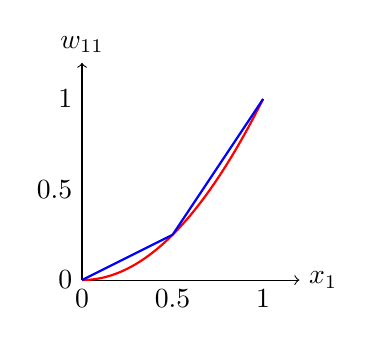
\begin{tikzpicture}[scale=2.3]


\draw[->] (0, 0) -- (1.2, 0) node[right] {$x_1$};
\draw[->] (0, 0) -- (0, 1.2) node[above] {$w_{11}$};
\draw[domain=0:1, smooth, variable=\x, red, thick] plot ({\x}, {\x*\x});
% \draw[domain=0:0.3, smooth, variable=\x, blue, thick] plot ({\x}, {0.3*\x});
% \draw[domain=0.3:0.6, smooth, variable=\x, blue, thick] plot ({\x}, {0.9*\x - 0.18});
% \draw[domain=0.6:1, smooth, variable=\x, blue, thick] plot ({\x}, {1.6*\x - 0.6});
\draw[domain=0:0.5, smooth, variable=\x, blue, thick] plot ({\x}, {0.5*\x});
\draw[domain=0.5:1, smooth, variable=\x, blue, thick] plot ({\x}, {1.5*\x - 0.5});

\node at (0,0) [below] {$0$};
\node at (0.5,0) [below] {$0.5$};
\node at (1,0) [below] {$1$};
\node at (0,0) [left] {$0$};
\node at (0,0.5) [left] {$0.5$};
\node at (0,1) [left] {$1$};

\end{tikzpicture}


% \caption{Piecewise McCormick relaxation for a quadratic term}
\end{subfigure}
\caption{
% Visualizing the Piecewise McCormick Relaxations for a bilinear and a univariate quadratic term. 
The left and middle plots illustrate the lower and upper parts, respectively, of the piecewise McCormick relaxation for the bilinear term \mbox{$w_{12} = x_1 x_2$} on the domain $x_1, x_2 \in [-1,1]$ (domain changed from $[0,1]$ for better illustration) with partitions \mbox{$\mathcal{P}_1 = \mathcal{P}_2 = [-1,0,1]$}.
% The right plot illustrates the piecewise McCormick relaxation for the quadratic term $w_{11} = x^2_1$ on the domain $x_1 \in [0,1]$ (the lower part coincides with the red curve) with the partition $\mathcal{P}_1 = \{0,0.3,0.6,1\}$.
The right plot illustrates the piecewise McCormick relaxation for the quadratic term $w_{11} = x^2_1$ on the domain $x_1 \in [0,1]$ (the lower part coincides with the red quadratic curve) with the partition $\mathcal{P}_1 = [0,0.5,1]$.
}
\label{fig:piecewise_mccormick}
\end{figure}